% !TEX program = lualatex
\documentclass[a4paper,10pt,oneside,openany]{ltjsreport}
\usepackage[margin=21mm,top=19mm,bottom=20mm]{geometry}
\usepackage[haranoaji]{luatexja-preset}
\usepackage{amsmath,amssymb,graphicx,booktabs,longtable,xcolor,float}
\usepackage[unicode,colorlinks=true,linkcolor=blue!45!black,urlcolor=blue!45!black]{hyperref}
\usepackage{caption}
\captionsetup{font=small,labelfont=bf}
\setcounter{tocdepth}{0}
\setlength{\parskip}{0.45em}
\setlength{\parindent}{1em}
\raggedbottom
\newcommand{\sourcefile}[1]{{\small\texttt{\detokenize{#1}}}}
\begin{document}


\title{\Huge 実験2\\[0.6em]\LARGE 半充填における反強磁性状態\\[1em]\large 一次元HubbardモデルのUHF計算}

\author{保存結果の解析レポート}\date{2026年11月2日}\maketitle

\chapter*{概要}

半充填、$U=4$、$N_\uparrow=N_\downarrow=25$ の系を反強磁性型初期密度から計算した。両境界条件とも126反復で収束し、電荷密度は一様、局所磁化は交互符号を持つ。これはUHF近似で得た対称性の破れた自己無撞着解であり、厳密な一次元多体系の磁気秩序を直接証明する結果ではない。

対象は2ケース、保存図9枚である。収束は2ケース、未収束は0ケース。本書では生成物の種類ごとに章を設け、同じ条件のOBCとPBCを並べて読む。

\tableofcontents

\chapter{計算ログ：条件と最終結果}

\sourcefile{uhf_results.txt}

\section*{計算条件と量の定義}

$L=50$、$t=1$、温度 $T=0$、外部電場なし。全エネルギーと軌道エネルギーは $t$ を単位とする。
OBCは開放端、PBCはサイト50と1も接続する周期境界である。$N_e=N_\uparrow+N_\downarrow$、$\Delta N=N_\uparrow-N_\downarrow$ と定義する。
収束判定は混合前の密度残差 $r<10^{-10}$、最大反復回数は10000である。
表の「未」は未収束の最終再評価値であり、その桁数は精度保証ではない。

\begin{center}\small\setlength{\tabcolsep}{4pt}
\begin{longtable}{lrrrr}
\toprule
条件 & $N_e$ & $\Delta N$ & $U/t$ & mixing \\ \midrule
\endhead
基準 & 50 & 0 & 4 & 0.25 \\
\bottomrule\end{longtable}\end{center}

\section*{最終エネルギー}

$E=E_{\rm kin}+E_{\rm int}$、$E_{\rm int}=U\sum_i n_{i\uparrow}n_{i\downarrow}$。全エネルギーは占有軌道固有値の単純な総和ではなく、平均場の二重計数を除いた量である。

\begin{center}\small\setlength{\tabcolsep}{4pt}
\begin{longtable}{lrrrr}
\toprule
条件/境界 & 状態 & $E$ & $E_{\rm kin}$ & $E_{\rm int}$ \\ \midrule
\endhead
OBC & 収束 & -23.013070704 & -43.110712440 & 20.097641737 \\
PBC & 収束 & -23.455261995 & -43.889991764 & 20.434729770 \\
\bottomrule\end{longtable}\end{center}

半充填、$U=4$、$N_\uparrow=N_\downarrow=25$ の系を反強磁性型初期密度から計算した。両境界条件とも126反復で収束し、電荷密度は一様、局所磁化は交互符号を持つ。これはUHF近似で得た対称性の破れた自己無撞着解であり、厳密な一次元多体系の磁気秩序を直接証明する結果ではない。

\section*{原資料と再利用}

出典は \sourcefile{results_vault/experiment_02/} 内の各条件/OBC・PBCのログ、CSV、PNG。\\ 補助資料は \sourcefile{experiment_conditions.md} と \sourcefile{uhf.jl}。値は保存済みの結果から採り、SCFを再実行していない。

条件名は原資料のディレクトリ名である。本実験は新規計算の結果のみである。

再利用データは独立した追加試行ではない。本書の解釈は保存された有限サイズ・UHF解の範囲に限る。

\chapter{密度CSV：電荷分布と二重占有}

\sourcefile{density_checkpoint.csv}

CSVの50サイトすべてから $q_i=n_{i\uparrow}+n_{i\downarrow}$、$m_i=n_{i\uparrow}-n_{i\downarrow}$、
$D=L^{-1}\sum_i n_{i\uparrow}n_{i\downarrow}$ を計算した。密度の各スピン成分は0以上1以下で、総和は指定した粒子数に一致することを確認した。未収束時のCSVは最後の混合密度を対角化して得た出力密度であり、固定点の密度とは限らない。

\begin{center}\small\setlength{\tabcolsep}{4pt}
\begin{longtable}{lrrrr}
\toprule
条件/境界 & 状態 & $\min q_i$ & $\max q_i$ & $D$ \\ \midrule
\endhead
OBC & 収束 & 1.000000 & 1.000000 & 0.100488 \\
PBC & 収束 & 1.000000 & 1.000000 & 0.102174 \\
\bottomrule\end{longtable}\end{center}

電荷密度は $q_i=1$ を保ち、スピン密度だけが交互に変調する。PBCの磁化振幅はほぼ一様である一方、OBCでは端で大きい。平均二重占有 $D$ は密度積から求めるUHFの値であり、厳密解の相関関数ではない。

\chapter{SCFエネルギー：反復による変化}

\sourcefile{scf_energy.png}

初期の数十反復でエネルギーの大部分が低下し、その後は図上ほぼ平坦となる。PBCの運動エネルギーはOBCより約0.779279低いが、相互作用エネルギーは約0.337088高い。両者の差し引きが全エネルギー差 $-0.442191290827$ を与える。単に相互作用エネルギーだけが小さい状態を選ぶわけではない。

各図の横軸は反復回数、縦軸は各反復で評価した全エネルギーである。図ごとに軸範囲が異なるため、見かけの傾きだけを比較しない。最終ログ値は反復終了後の再評価であり、履歴の最終点とわずかに異なる場合がある。

\begin{center}\small\setlength{\tabcolsep}{4pt}
\begin{longtable}{lrrr}
\toprule
条件/境界 & 初回 $E$ & 最終 $E$ & 最後の履歴の $|\Delta E|$ \\ \midrule
\endhead
OBC & -17.140038 & -23.013071 & $0$ \\
PBC & -17.699645 & -23.455262 & $0$ \\
\bottomrule\end{longtable}\end{center}

\begin{figure}[H]\centering

\begin{minipage}{0.49\linewidth}\centering

\textbf{OBC：収束}\par

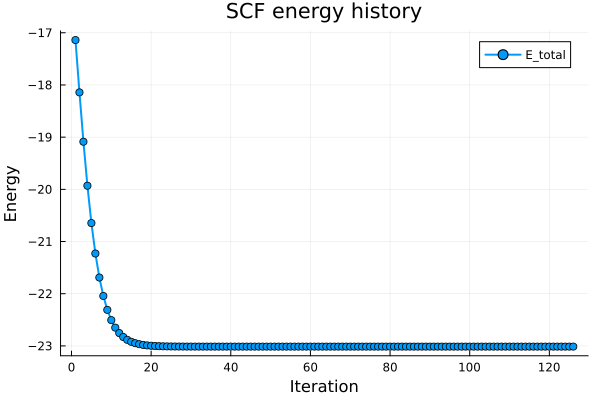
\includegraphics[width=\linewidth]{../../results_vault/experiment_02/OBC/scf_energy.png}

\end{minipage}\hfill%
\begin{minipage}{0.49\linewidth}\centering

\textbf{PBC：収束}\par

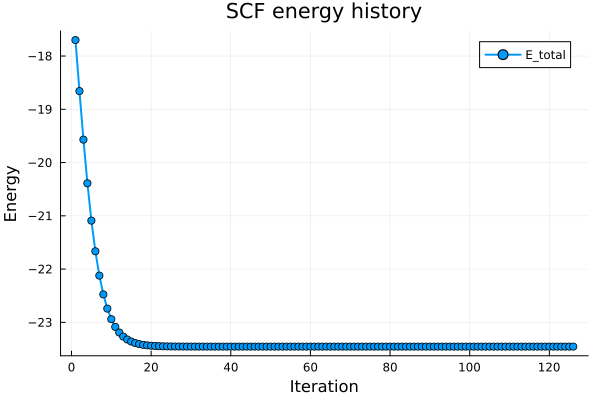
\includegraphics[width=\linewidth]{../../results_vault/experiment_02/PBC/scf_energy.png}

\end{minipage}

\caption{基準条件。SCFエネルギーの比較。左：OBC、右：PBC。}\end{figure}

\chapter{SCF残差：自己無撞着性}

\sourcefile{scf_residual.png}

残差は後半に対数軸でほぼ直線的に減少する。OBCとPBCで反復回数は同じで、最終残差はいずれも約 $3.26\times10^{-11}$ である。エネルギーの見た目の平坦化より遅く密度の自己無撞着条件が満たされる。

残差は $r=\max_{i,\sigma}|F[n]_{i\sigma}-n_{i\sigma}|$。表は最終再評価値である。収束時には出力密度を採用してから再評価するため、履歴図の最後の残差とは同じとは限らない。

\begin{center}\small\setlength{\tabcolsep}{4pt}
\begin{longtable}{lrrr}
\toprule
条件/境界 & 状態 & 反復数 & 最終残差 \\ \midrule
\endhead
OBC & 収束 & 126 & $3.266\times10^{-11}$ \\
PBC & 収束 & 126 & $3.263\times10^{-11}$ \\
\bottomrule\end{longtable}\end{center}

\begin{figure}[H]\centering

\begin{minipage}{0.49\linewidth}\centering

\textbf{OBC：収束}\par

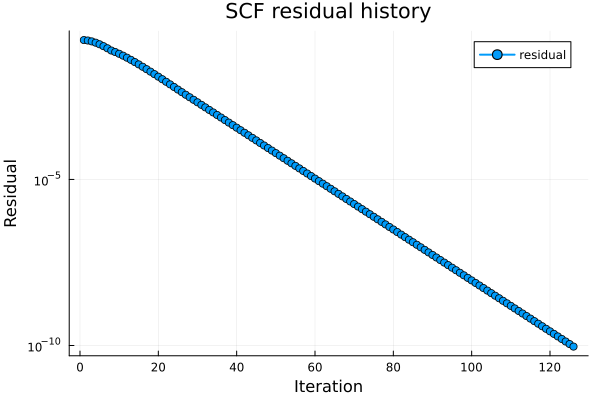
\includegraphics[width=\linewidth]{../../results_vault/experiment_02/OBC/scf_residual.png}

\end{minipage}\hfill%
\begin{minipage}{0.49\linewidth}\centering

\textbf{PBC：収束}\par

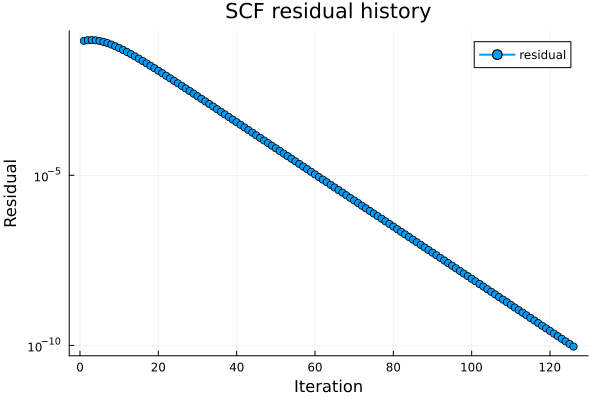
\includegraphics[width=\linewidth]{../../results_vault/experiment_02/PBC/scf_residual.png}

\end{minipage}

\caption{基準条件。SCF残差の比較。左：OBC、右：PBC。}\end{figure}

\chapter{軌道エネルギー：準位構造}

\sourcefile{final_orbital_energies.png}

上下スピンは局所密度が異なっていても、固有値の曲線は重なっている。25番目と26番目の間に大きな準位の分離があり、反強磁性平均場と整合する。PBCの階段状の縮退とOBCの滑らかな準位列には有限鎖の違いが残る。横軸は波数ではないので、この図をそのままバンド分散とは呼べない。

横軸はエネルギー昇順の軌道番号、縦軸は $h_\sigma=h_0+U\operatorname{diag}(n_{\bar\sigma})$ の固有値である。固有値の数値ファイルは保存されていないため、図からの解釈は定性的なものに留める。未収束例をCSVから再対角化すると保存図とは異なる平均場になる可能性があり、本書ではその置換を行わない。

\begin{figure}[H]\centering

\begin{minipage}{0.49\linewidth}\centering

\textbf{OBC：収束}\par

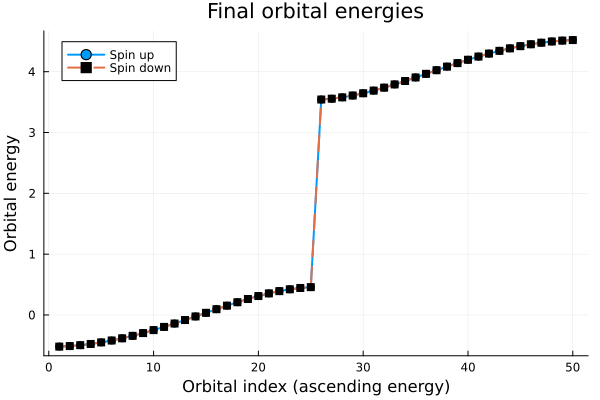
\includegraphics[width=\linewidth]{../../results_vault/experiment_02/OBC/final_orbital_energies.png}

\end{minipage}\hfill%
\begin{minipage}{0.49\linewidth}\centering

\textbf{PBC：収束}\par

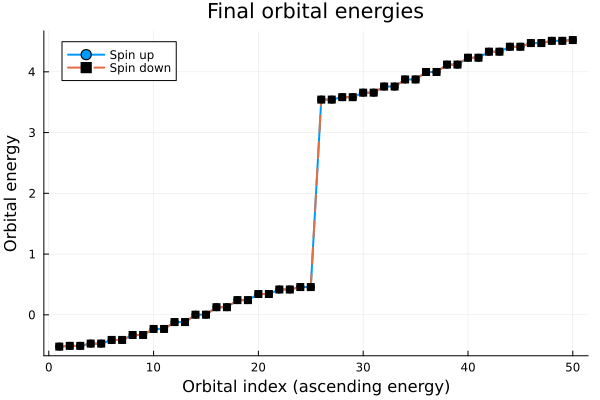
\includegraphics[width=\linewidth]{../../results_vault/experiment_02/PBC/final_orbital_energies.png}

\end{minipage}

\caption{基準条件。軌道エネルギーの比較。左：OBC、右：PBC。}\end{figure}

\chapter{局所磁化：空間構造}

\sourcefile{final_magnetization.png}

PBCでは $|m_i|\simeq0.768964$ が全体に続く。OBCでは端の $|m_1|\simeq0.87559$ が中央の約0.76896より大きい。開放端で隣接結合が減ることに伴う磁化の増強と解釈できる。$\sum_i m_i=0$ でも局所磁化は消えておらず、全磁化と反強磁性秩序を区別する必要がある。

$\overline{|m|}=L^{-1}\sum_i|m_i|$、$M_{\rm AF}=|L^{-1}\sum_i(-1)^im_i|$ と定義する。$m_i$ はスピン密度差であり、$\langle S_i^z\rangle=m_i/2$ に対応する。全磁化は $\sum_i m_i=\Delta N$ と粒子数制約で固定される。

\begin{center}\small\setlength{\tabcolsep}{4pt}
\begin{longtable}{lrrr}
\toprule
条件/境界 & 状態 & $\overline{|m|}$ & $M_{\rm AF}$ \\ \midrule
\endhead
OBC & 収束 & 0.773051 & 0.773051 \\
PBC & 収束 & 0.768964 & 0.768964 \\
\bottomrule\end{longtable}\end{center}

\begin{figure}[H]\centering

\begin{minipage}{0.49\linewidth}\centering

\textbf{OBC：収束}\par

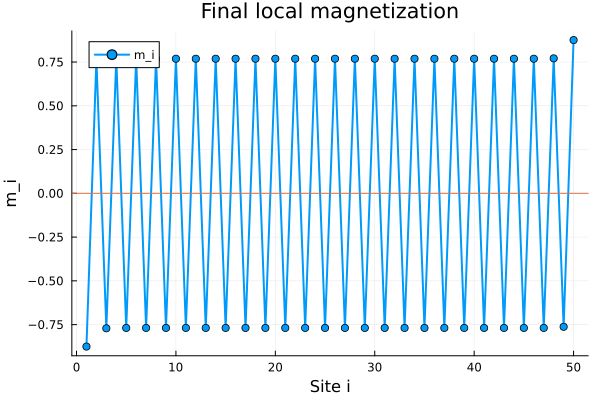
\includegraphics[width=\linewidth]{../../results_vault/experiment_02/OBC/final_magnetization.png}

\end{minipage}\hfill%
\begin{minipage}{0.49\linewidth}\centering

\textbf{PBC：収束}\par

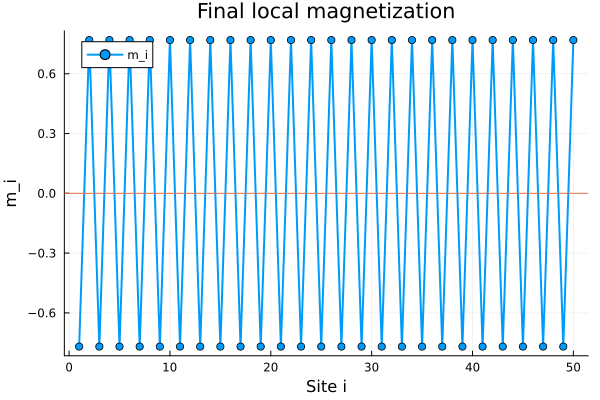
\includegraphics[width=\linewidth]{../../results_vault/experiment_02/PBC/final_magnetization.png}

\end{minipage}

\caption{基準条件。局所磁化の比較。左：OBC、右：PBC。}\end{figure}

\chapter{境界条件による全エネルギー差}

\sourcefile{boundary_energy_difference.png}

$\Delta E_{\rm boundary}=E_{\rm PBC}-E_{\rm OBC}$ と定義する。負ならPBC、正ならOBCの保存された解の方が低エネルギーである。両方が収束した組だけを表と図で数値比較し、それ以外をNCとする。

PBCの方が0.442191低い。非相互作用の実験1での差0.758400より絶対値が小さく、相互作用による密度の再配列が境界条件の効果を変えている。同じ条件内で比較した差であり、異なる $U$ の全エネルギー順位を相の安定性の比較に使うものではない。

\begin{center}\small\setlength{\tabcolsep}{4pt}
\begin{longtable}{lrr}
\toprule
条件 & $\Delta E_{\rm boundary}$ & $\Delta E_{\rm boundary}/L$ \\ \midrule
\endhead
基準 & -0.442191290827 & -0.008843825817 \\
\bottomrule\end{longtable}\end{center}

\begin{figure}[H]\centering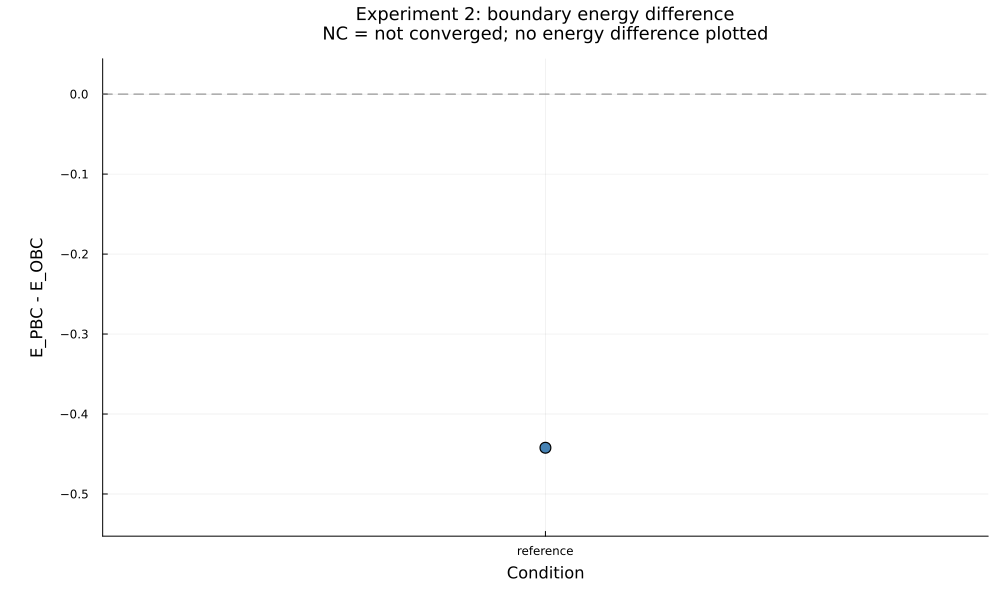
\includegraphics[width=0.9\linewidth]{../../results_vault/experiment_02/boundary_energy_difference.png}\caption{保存済みの境界エネルギー差。NCは未収束の組を示し、差が0であることを意味しない。}\end{figure}

\section*{結論と残された確認}

半充填、$U=4$、$N_\uparrow=N_\downarrow=25$ の系を反強磁性型初期密度から計算した。両境界条件とも126反復で収束し、電荷密度は一様、局所磁化は交互符号を持つ。これはUHF近似で得た対称性の破れた自己無撞着解であり、厳密な一次元多体系の磁気秩序を直接証明する結果ではない。

対象ケースはすべて収束した。ただし、収束判定だけでは得られた解が大域的な最小エネルギー状態であることまでは保証されない。

サイズは50に固定しているため、境界効果と有限サイズ効果の切り分けには別サイズの結果が必要である。

\end{document}